\documentclass[12pt,a4paper,twoside]{report}
\usepackage[german,english]{babel}
\usepackage[latin1]{inputenc}
\usepackage{amsfonts}
\usepackage{amsmath}
\usepackage{amssymb}
\usepackage{capt-of}
\usepackage{epsfig}
\usepackage{moreverb}
\usepackage{rotating}
\usepackage{enumerate}
\usepackage{graphics, graphicx,wrapfig}
\usepackage{fancybox}
\usepackage{picinpar,varioref,floatflt}
\usepackage{ae}
\usepackage{longtable}
\usepackage{textcomp}
\usepackage{unizhtr}
\usepackage{chapterbib}
\usepackage{minitoc}
\usepackage{float}
\usepackage{url}
\usepackage[]{siunitx}
\usepackage{placeins}



\renewcommand{\mtctitle}{Contents}
\setcounter{tocdepth}{0}
\pagestyle{myheadings}

\selectlanguage{english}

\begin{document}
\dominitoc

\textheight240mm
\setlength{\oddsidemargin}{4mm}
\setlength{\evensidemargin}{-5.5mm}
\topmargin-6.0mm
\setlength{\parindent}{0ex}
\setlength{\parskip}{2.0ex plus 0.9ex minus 0.4ex}
\setcounter{secnumdepth}{3}

\tableofcontents
\cleardoublepage

\chapter{Security Policy Reconfiguration Solutions in Wireless Sensor Networks}
\markboth{Security Policy Reconfiguration Solutions in Wireless Sensor Networks}{}
\chaptauthors{Anastasia Ruvimova, Raphael Ochsenbein, Sanjiv Jha}


\Kurzfassung{%
This is the abstract.
It fits pretty much on one page and is definitely not longer.}

\newpage

\minitoc %table of contents

\newpage

\section{Introduction}
A Wireless Sensor Network(WSN) is a collection of distributed autonomous sensors to monitor physical or environmental conditions, such as temperature, sound, pressure, gases, etc. and to cooperatively pass their data through the network to a decision maker's location. for an example Intelligent Transport System, it is One of the most relevant applications today, where the security issues in Wireless Sensor Networks play a very important role. These systems have the potential to improve mobility, safety and security, while ensuring energy efficiency and reducing the environmental impact of transportation systems. \par
The recent technology revolution has made the WSN to be employed on large scale. These networks have myriad of sensors and many different types of Sensors are being used for different scenarios. The example could be the military, traffic control, healthcare, environment monitoring and in the field of farming too they are being used. The implementation of WSN has increased in the number, so has the security attacks. To make the network secure and reliable, different security policies are needed to be implemented. To make network more robust and achieve required security, the network is composed of many different types of sensors. As the heterogeneity of sensors increases the security policies at each node increases. These different types of node are constraint with the constituting parts as OS, restricted memory and processing power. Thus, the generic security policies are not applicable for each node, as all have different configuration and requirements.\par
The Intelligent Transport Systems are composed of different kinds of devices installed at several locations, such as sensors inside the vehicles and sensors on the traffic signals. For instance, the vehicles can be equipped with several sensors with different sensor units, such as acoustic, accelerometers, temperature, the vehicle's on-board unit (OBU) computers, and GPS devices. These sensors are used to ensure safe driving, being responsible, for instance, for measuring the distance to obstacles around them. The vehicles also use information received from surrounding vehicles, such as their speed or distance, and are able to communicate with each other in order to cooperate for safety and other reasons. Furthermore, the traffic signals send information to the vehicles informing them of speed limits and general traffic regulations.  Intelligent Transport Systems have a wide variety of interesting applications, such as road safety applications.\par
Use of myriad of sensors, increases the chances of communication disturbance and in other cases the information are highly confidential (e.g., research work satellite communication). The security needs of all of these applications are quite important. \par
In case of ITS, to know whether a node in the network is being uncooperative or malicious is really crucial to prevent intentionally wrong instructions being sent to a vehicle. Furthermore, these systems are very dynamic, and their contextual environment changes very frequently, so they need different security policies adapted to the changing environment. The Intelligent Transports System (ITS) infrastructure is composed of extremely heterogeneous devices where both the monitoring and the deployment and management of the security policies must be performed in different ways.
\begin{figure}[ht]
	\begin{center}
  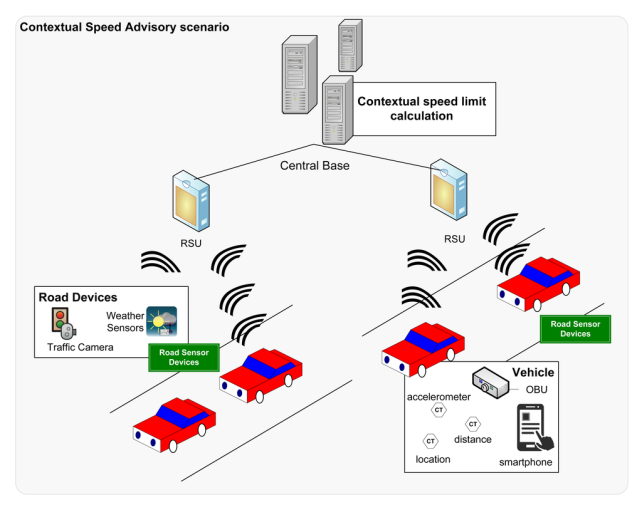
\includegraphics[width=0.6\textwidth,natwidth=652,natheight=510]{./figures/figure-01.png}
  \end{center}
  \caption{A context speed advisory (CSA) scenario \cite{Pinto;etal:2013}}.
  \label{fig:label}
\end{figure}

In ITS, WSN (A context speed advisory scenario Figure 1.1) is used to indicate that the recommended the speed when you have traffic congestion in the vicinity could cause an accident. Therefore, the messages sent between the nodes and the base station must be properly encrypted, and all of the nodes must be trustworthy. Therefore, the self-protection of the whole system is required. However, very hard security policies have a penalty in efficiency, especially in energy and performance, two typical requirements of these applications. Therefore, the security policy to be applied in each situation must be negotiated to make a balance between the necessary security and the efficiency. Additionally, as these situations can change quickly, these policies have to be (re)negotiated. For instance, in the case where malicious software is suspected in a given WSN (detected by intruder detection algorithms), the security needs to be increased, and the suspect nodes must be isolated. To the contrary, on roads where the main interest is to preserve the lifetime of the system and there is no risk of malicious attacks, the security can be a little bit weaker. Similarly, in situations where communication performance is required (e.g., high traffic density) the security could also be relaxed. On the other hand, in exceptional circumstances, the interception of data sent by certain vehicles (e.g., a presidential motorcade) has to be totally avoided. In this case, the security policy applied to these specific nodes must be modified.\par
There are some important effort being made to develop specific algorithm for WSNs in the fields of trust, security and privacy, such as new algorithms for authentication, positioning, network intrusion detection, efficient key management for dynamic Wireless sensor networks, etc. As a network has many different sensors with different requirements. If the same algorithm has been implemented in all the nodes and the working environment has changed, the present algorithms for some specific nodes needs improvement,i.e, new algorithms are to be implemented within the nodes to work in the changed environment, which was not mainly done by the previous algorithm. So, the nodes have to be adaptive to change accordingly. The main issues captured in the new advanced algorithm are low-level programming abstractions, limited capabilities, different routing protocols,etc. Now as the sensor nodes need to be adaptive to the environment change with the lowest impact for users and without stopping the devices. In addition to it, it is needed to adapt the specific algorithm as required.\par
The rest of the paper is organized as follows. After this Introduction, Section 2 Discusses different Security Considerations in WSNs with the Security Vulnerabilities and Defense Strategies for WSNs. Section 3 presents three different solutions or Use Cases for Security Re-configuration in WSNs. In further Section 4 The paper Evaluates the Challenges and Approaches for Inter-trust \& FamiWare, and we present our Conclusions and the last section 5, gives the list of Acronyms and Terminologies used throughout the paper.  \par
\section{Security Considerations in WSNs}
In this section we analyze known Denial of Service (DoS) threats and attacks on privacy and authentication on the four primary levels: the physical layer, link layer, network layer, and transport layer. 
\subsection{Security Vulnerabilities in WSNs}
For many of the before mentioned WSN applications, security is of very high priority. WSNs are often deployed in remote locations and left unattended (for example, sensors which watch for fire activity in forests) and are, therefore, especially vulnerable to attacks. Unfortunately, the resource constraints of these sensors do not allow for traditional high-overhead security mechanisms. We will propose several solutions after analyzing the threats we need to protect against. \par
These attacks may be categorized into attacks on security and authentication and DoS attacks. Attacks on security and authentication include packet modification, eavesdropping, and spoofing of packets. As described by Sen, DoS attacks "may permit real-world damage to the health and safety of people. The DoS attack usually refers to an adversary's attempt to disrupt, subvert, or destroy a network. However, a DoS attack can be any event that diminishes or eliminates a network's capacity to perform its expected functions" \cite{sen:2009}.\par
\subsubsection{DoS Attacks}
DoS attacks in WSNs are sometimes very costly and have received much attention from researches. These attacks exist on four levels: the physical layer, the link layer, the network layer, and the transport layer. We will analyze the threats for each in the following. \par\par
The physical layer is responsible for "frequency selection, carrier frequency generation, signal detection, modulation, and data encryption" \cite{sen:2009}. These attacks are especially threatening because WSNs may be deployed in hostile environments where an attacker has physical access. The two types of attacks on the physical layer are jamming and tampering. The first attack, jamming is defined as an attack which interferes with the node's radio frequencies used for communication. Even intermittent jamming may prove destructive as messages in network communication are often time-sensitive.  A jamming source may disrupt the entire network. \par
Because sensor networks are often deployed in remote outdoor environments and left unattended, nodes are also highly vulnerable to tampering. Sen warns that "physical attacks may cause irreversible damage to the nodes. The adversary can extract cryptographic keys from the captured node, tamper with its circuitry, modify the program codes or even replace it with a malicious sensor. It has been shown that sensor nodes such as MICA2 motes can be compromised in less than one minute time" \cite{sen:2009}.  \par\par
The next level up, the link layer, is responsible for multiplexing of data-streams, data frame detection, medium access control, and error control. This layer is vulnerable to attacks which include: resource exhaustion, purposefully created collisions, and unfairness in allocation \cite{sen:2009}. A collision is defined as an attack where two nodes attempt to transmit on the same frequency simultaneously, causing the packets to be discarded and require retransmission. Sen elaborates on these attacks, noting that: "an adversary may strategically cause collisions in specific packets such as ACK control messages. A possible result of such collisions is the costly exponential back-off. The adversary may simply violate the communication protocol and continuously transmit messages in an attempt to generate collisions" \cite{sen:2009}. \par
Strategically-placed collisions may also result in resource exhaustion, for example: when a naive link layer node continuously attempts to retransmit the corrupted packets. The third attack, unfairness of allocation is a weak form of DoS attack caused by intermittently employing collision and resource exhaustion: "the adversary causes degradation of real-time applications running on other nodes by intermittently disrupting their frame transmissions" \cite{sen:2009}. \par\par
Attacks on the network layer of WSNs include spoofed routing information, selective packet forwarding, sinkhole, Sybil, wormhole, hello flood, acknowledgment spoofing, and more. A brief description of these attacks follows. \par
The first, spoofed routing information directly targets the network's routing information by altering, spoofing, or replaying routing information to disrupt the network's traffic \cite{sen:2009}. As Sen describes, these disruptions include "creation of routing loops, attracting or repelling network traffic from selected nodes, extending or shortening source routes, generating fake error messages, causing network partitioning, and increasing end-to-end latency" \cite{sen:2009}. In a multi-hop network like a Wireless Sensor Network, all the nodes need to forward messages accurately for message communication. \par
An attacker may compromise this communication through selective forwarding, where some messages are forwarded and others are dropped. In a sinkhole attack, a node's routing information is altered to make it look more attractive than others. As a result, its neighbor nodes choose this compromised node for data routing. \par
In a sybil attack, a node is made to present multiple identities in the network, which disrupts the data distribution in peer-to-peer networks. Sen notes that "in addition to defeating distributed data storage systems, the Sybil attack is also effective against routing algorithms, data aggregation, voting, fair resource allocation, and foiling misbehavior detection." For example, may take on more than one identity in order to generate additional "votes". Similarly, the compromised node would use its multiple identities to route multiple paths through a single malicious node \cite{sen:2009}. \par
Our next attack is the wormhole - is a low latency link through which messages can be replayed between two parts of the network. This is similar to a sinkhole attack in that it creates a one-hop link to the base station through the attacking node in a far part of the network. \par
The hello flood attack abuses the common assumptions among Hello packet protocols that receiving a packet implies that the sender is within radio range of the receiver. The attacker can use a high-powered transmitter to fool many nodes into thinking they're within the neighborhood. As a result, the attacker broadcasts a shorter route to the base station and all the nodes which receive the Hello packet attempt to transmit to the attacker node, but the nodes are out of range. \par
Some algorithms for routing WSN's require acknowledgement packet transmission. We define acknowledgment spoofing as an attack where the malicious node overhears packet transmissions from its neighbor nodes and spoofs the acknowledgements, providing false data to the nodes. This results in false information being disseminated to the nodes. \par
\subsubsection{Transport Layer}
The Transport Layer is vulnerable to flooding attacks and desynchronization attacks. The flooding attack exhausts the node's memory by repeatedly making a new connection request until resources required by each connection have reached a maximum limit. Thus, further legitimate requests are ignored.\par
An attacker may use desynchronization by disrupting existing connections. This can be done by repeatedly spoofing messages to an end host, resulting in the request for retransmission of missed framed. The attacker may time this to hinder the end host's ability to exchange data, causing them to waste energy attempting to recover from errors which do not exist. \par
To summarize, we list the layers and their respective attack vulnerabilities below. \par
\FloatBarrier
  \begin{table}[h]
  	\begin{center}
    \begin{tabular}{|c|c|} \hline
	        Layer & Attack \\ \hline\hline
	        Physical Layer & Jamming, tampering \\ \hline
	        Link Layer & Collision, resource exhaustion, unfairness in allocation \\ \hline
	        Network Layer & \shortstack{Spoofed routing information, \\selective packet forwarding, sinkhole,\\ Sybil, wormhole, hello flood, \\acknowledgement spoofing} \\ \hline
	        Transport Layer & Flooding, de-synchronization \\ \hline
	  \end{tabular}
	  \end{center}
  \end{table}
\FloatBarrier
\subsubsection{Attacks on Privacy}
Let us now analyze attacks on secrecy and authentication. We begin with the node replication attack in which an attacker copies a node into the network by replicating an existing node's identifier. This node copy may cause severe damage to the communication by corrupting and forwarding the packets in wrong routes. Sen adds that "this may also lead to network partitioning, communication of false sensor readings. In addition, if the attacker gains physical access to the entire network, it is possible for him to copy the cryptographic keys and use these keys for message communication from the replicated node. The attacker can also place the replicated node in strategic locations in the network so that he could easily manipulate a specific segment of the network, possibly causing a network partitioning" \cite{sen:2009}.\par
In addition to DoS attacks, WSNs are vulnerable to attacks on privacy and authentication. This is partially a side effect of the network's ability to automate data collection through efficient sensor deployment. Unfortunately, protecting sensitive data in wireless networks is no easy task. This is especially so because seemingly innocuous data might give the attacker enough material to derive sensitive data. Moreover, a large amount of data is easily accessible through remote access mechanisms, so the attacker does not need to be present to get his or her hands on the data and may remain anonymous. The adversary may even monitor several sites at once.  We will take a look at a few common attacks on sensor data privacy.\par
The simplest and most common attack on information privacy is eavesdropping and passive monitoring. Without cryptographic protection, the attacker can easily understand the contents. Sen warns, "packets containing control information in a WSN convey more information than accessible through the location server. Eavesdropping on these messages prove more effective for an adversary" \cite{sen:2009}. For even more effectiveness, eavesdropping can be combined with traffic analysis. If done right, the adversary can pick out nodes which have special roles and activities in the network. For example, "a sudden increase in message communication between certain nodes signifies that those nodes have some specific activities and events to monitor" \cite{sen:2009}. \par
The attacker may use camouflage by compromising a senor node in the network and later using it to masquerade as a normal node. This false node may send false routing information and attract packets from other nodes to forward further. Having received the packets, the node forwards them to strategic nodes where privacy analysis is carried out systematically on the packets. As seen above, wireless sensor networks are subject to threats on many levels and by numerous approaches, making it even more difficult to find a universal security policy.\par

\subsection{Defense Strategies for WSNs}
\subsubsection{Cryptography and Key Management}
In the previous section, a host of attack vectors on WSNs have been described. For most of these vectors, there exist various defense, or at least mitigation mechanisms which can, in combination with each other, be used to protect wireless sensor networks. However, due to the limited resources of the sensor nodes,  the defense mechanisms have to be employed strategically so as to not overuse the computing power and run into run-time performance problems and to prevent overly consuming the battery power of the device.\par
This performance dilemma may be most striking, when evaluating the cryptographic algorithms to be deployed in the network: many researchers are hesitant in recommending public key cryptography for sensor networks, as the code \& data size as well as the computational and energetic load are too high for sensor nodes \cite[ pp. 59]{sen:2009}. One experiment shows that encrypting 1kb consumes 42mJ when using an RSA public key  algorithm, whereas by using an AES encryption, slightly less than 1mJ is consumed \cite[ pp. 59]{sen:2009}. Only recently researchers have published proof that some public key cryptographic algorithms are suitable for deployment in WSNs. While the optimizations that can be used to deploy public key cryptography in WSNs will be demonstrated in the practical section of this paper, one main limitation should be noted here: the focus has mainly been on optimizing the public key operation time, and relies on nodes with more computational power for the private key operations, which still remain expensive \cite[ pp. 59]{sen:2009}. Therefore, these approaches might be less suitable for homogeneous sensor networks. Notably, the following algorithms have been shown to work in WSNs: Rabin's Scheme \cite{rabin:1979}, Ntru-Encrypt \cite{hoffstein;etal:1998}, RSA \cite{RSA:1983}, and Elliptic Curve Cryptography (ECC)\cite{miller:1986} \cite{kobiltz:1987}.\par
As an alternative to public key cryptography is found in symmetric key cryptography, and consequently a lot of research focuses on these algorithms for the encryption of sensitive data in sensor networks. With these methods, a single shared key is used between the nodes talking to each other and one of the key challenges is the distribution of said key \cite[ pp. 60]{sen:2009}. For this, it might be interesting to consider a hybrid approach, where a public key of the network key distribution center (KDC) is distributed to the sensor nodes, and the shared key for symmetric cryptography is distributed via public key cryptography.\par
A common approach in WSNs is to have the usually more powerful base station become the KDC for the network, as that usually requires keeping track of nodes and their keys, blacklisting keys in case a node corruption is detected \cite[ pp. 60]{sen:2009}. However, the drawback of this approach is that the base station becomes a single point of failure for the network.\par
There are several approaches, with which a KDC can manage the network keys and encryption based on heuristics. As described earlier, one might distinguish between more sensitive traffic, such as symmetric key exchanges, which requires stronger encryption. In a deterministic approach, there are predefined encryption mechanisms for different packets. On the other hand, a probabilistic and distributed schemes might be chosen \cite[ pp. 61]{sen:2009}. For instance, a random subset of a key ring can be shared with a number of nodes, which just have to find one common key to encrypt their communications. Furthermore, the subset of keys available to a node can be used as a fingerprint to identify a node \cite[ pp. 62]{sen:2009}.\par
\subsubsection{Protecting Against Denial-of-Service attacks}
Since a Denial of Service (DoS) attack can occur on multiple network layers, barriers also have to be established on each layer that can be attacked. At the same time defending against these attacks is very costly, and it should be assumed that a determined attacker will always be able to mount an attack with enough processing power to overpower the capabilities of sensor nodes. In light of this, mitigation strategies are useful in limiting the impact and damage that can easily be inflicted in WSNs.\par
Within the physical network layer, a jamming attack can be prevented by such mechanisms as frequency hopping and code spreading, and more generally by spread-spectrum communication \cite[ pp. 64]{sen:2009}. Unfortunately these techniques require more complex design and consume more energy, making a defense of the physical network layer impractical for many applications of WSNs.\par
Against collision attacks in the link layer, a preferred defense mechanism would be the use of error-correcting codes, which also work for mitigating environmental or probabilistic errors \cite[ pp. 64]{sen:2009}. The drawback of these codes is that they add to the processing overhead during communication, and according to Sen, there is currently no complete defense against collision attacks available \cite[ pp. 64]{sen:2009}.  In order to protect against the selective forwarding attack, it is possible to send data over multiple paths \cite[ pp. 65]{sen:2009}. One novel approach to defend against flooding DoS attacks put forward by researchers is to require that clients solve a puzzle when connecting, in order to demonstrate their willingness to contribute to the network \cite[ pp. 65]{sen:2009}. As with many other solutions, this puts a greater burden on the client, which might not be desirable for certain low-power use cases. The last defense mechanism in the link layer is to secure that the multicast and broadcast messages cannot be intercepted by unauthorized third parties \cite[ pp. 65]{sen:2009}. \par
\subsubsection{Protecting Against Routing Protocol Attacks}
Securing the routing protocol has the main goal of ensuring the integrity, authenticity and correct transmissal of messages in the network \cite[ pp. 66]{sen:2009}. Consequently, this means securing all of the traffic in the network with one of the previously described encryption algorithms. There exist a number of secured routing protocols which can be used to secure the sensor network. \par
The first routing protocol is \si{micro}TESLA (the micro version of the timed efficient streaming loss-tolerant authentication protocol), another protocol is INENS (intrusion tolerant routing protocol in wireless sensor networks), yet another protocol is SNEP (secure network encryption protocol), and there is also TRANS (trust routing for location aware sensor networks); additionally there are protocols built upon the other protocols, such as SPINS which incorporates \si{micro}TESLA and SNEP \cite[ pp. 67-68]{sen:2009}\par
\subsubsection{Defense Against the Sybil Attack}
In order to protect against the sybil attack, it's necessary that the nodes of the network can be correctly identified, and that every node exists only once. In other words, the network needs to be capable of identifying fake / multiplied nodes, for instance by keeping track of all the network nodes and their respective keys and identities. This can be achieved either by having specific keys for each node, or by assigning different radio channels to nodes in the neighborhood and listening to those channels \cite[ pp. 68]{sen:2009}. In networks with random key predistribution, it's possible to use the keyring of a node to identify the node.\par
\subsubsection{Managing the Node Replication Attack}
Because centralized node identity management through the KDC or another central node has a single point of failure, and because distributed identity management protocols, such as neighborhood voting, would fail to detect distributed replications, collective identity verification algorithms have been brought forward. Both algorithms work by making a multicast to the network, which is then verified.\par
The first approach uses a randomized multicast of the node location to a randomly selected number of witnesses, whereby the number of  witnesses has to be chosen to be large enough to guarantee that in each neighborhood there are at least two witnesses \cite[ pp. 68]{sen:2009}. The number of witnesses can be calculated with the mathematics for the birthday paradox, which was originally used to calculate the probability of two people in a random group of people having the same birthday. Each node broadcasts it's location to the network, and each node stores the location information of it's neighbors. If a conflicting claim is found, the duplicate node is revoked \cite[ pp. 68]{sen:2009}. This method can find all duplicates in the network, if all the broadcasts reach all the nodes in the network, however this broadcast then introduces a high total communication cost for the network.\par
The second method uses the network topology and a line-selected multicast to detect replication. In order to reduce the communication overhead of the first multicast approach, every node chooses one random node as a witness which will keep track of the node's location \cite[ pp. 68]{sen:2009}. When the location is communicated to the witness, every node forwarding the information also keeps track of the location, and checks if there is any conflict. Therefore, if any node claims to be in an incorrect location,  as soon as the two paths for the location witness intersect, it's possible to detect the fraudulent claim.\par
\subsubsection{Preventing Traffic Analysis}
If the sensor network has a single base station or key distribution center, then the network has a single point of failure. An attacker might want to identify such a crucial device in the network, and to do so, traffic analysis would be one option. To defend against such an attack, first a multiple parent routing scheme should be introduced, where any node can forward packets to one of many parents \cite[ pp. 69]{sen:2009}. This creates a less deterministic network routing. Furthermore, the network hops towards the base station can be randomized through a controlled random walk. Additionally, random fake paths can be introduced, and fake communication hotspots / base stations can be added to the network. In combination, these methods together make it difficult to conduct traffic analysis for finding the base station.\par
\subsubsection{Protecting Sensor Privacy}
While encryption is one way to protect sensitive data, there is still a risk of the encrpytion being broken and the data being exposed. If the goal is to prevent the disclosure of sensitive data, even when encryption is broken, then it becomes necessary to strip identifying information from the data and make it anonymous. \par
The anonymization method that can be used to reduce the impact of a broken encryption key or a compromised node, is to store the sensitive data in a decentralized way in a tree structure over a range of nodes \cite[ pp. 69]{sen:2009}. In order to do calculations on the data, a number of nodes has to be involved collaboratively. In addition to that, the methods for preventing traffic analysis and routing protocol attacks should also be employed.\par
Another method to protect data is to manage access control by specifying several policies that restrict data access, with parameters such as time of request, location, speed, and identity \cite[ pp. 69]{sen:2009}. The drawback of using policies, however, is that they involve a server that enforces these policies, and therefore controls data access. Since it is impractical to enforce such policies on a node-level, again a single point for failure is introduced.\par
The next method for protecting sensitive data is information flooding. According to Sen, several flooding algorithm's of varying sophistication can be used \cite[ pp. 69]{sen:2009} The simplest approach is baseline flooding, where every node forwards the messages it receives only once, and never retransmits a message. To reduce the traffic, probabilistic flooding can be employed, where only a subset of nodes forward the data they receive. However, if an attacker intends to find the location of the source node, with the previous flooding algorithms, an attacker might be able to conduct traffic analysis in order to find the source node. Therefore, similar techniques as those preventing traffic analysis have to be employed for flooding as well. That means, fake messages have to be created, and the fake messages have to be created. However, here one does not only want to prevent finding the target of the traffic, but also the originator, and therefore phantom flooding should be used, which directs an attacker towards a fake source. To do so, first a random or directed walk to a phantom source is initiated, and the phantom source initiates a flooding request in order to deliver the message. Furthermore, the random walk has to be initiated from both source to sink, and from sink to source in order to prevent the collection of location information. To that end, the greedy random walk  (GROW) protocol can be used.\par
\subsubsection{Intrusion Detection}
In a widely deployed sensor network, it has to be assumed that some nodes can become compromised, especially so for low-power sensor nodes where less strict security mechanisms might be deployed due to computing and memory limitations of the node. For that reason, it becomes very important that the network has an intrusion detection system (IDS) in place, which can monitor the network for suspicious activity patterns and find corrupted or compromised nodes in order to revoke their network access \cite[ pp. 70]{sen:2009}.\par
One approach is to have an IDS implemented at node level, where the nodes do not exchange intrusion data, whereas in a second approach a cooperative IDS is implemented where each node has an intrusion detection agent to detect local attacks, but the intrusion data is exchanged between nodes in order to detect global attacks, and a third approach is to use a hierarchical architecture, where nodes are clustered and cluster heads manage the local traffic and intrusion detection for the cluster \cite[ pp. 70]{sen:2009}. One method to detect intrusion on a global is implemented with the interleaved hop-by-hop authentication (IHOP) scheme [141]. In order to detect local intrusion, a local intrusion detection system such as LIDS can be deployed on each node [5]. LIDS can also work on a global level, if the nodes collaborate to exchange security data and intrusion alerts amongst each other \cite[ pp. 71]{sen:2009}.\par
\subsubsection{Secure Data Aggregation}
With the goal of reducing unnecessary data transmission in order to save energy, many sensor networks make use of data aggregation at a level of node clusters. However, if such an cluster head is compromised, it becomes easy to either collect sensitive information and to inject false data in the network \cite[ pp. 71]{sen:2009}. However, there is a conflict between securing data aggregation and protecting data confidentiality, as in order to best aggregate data, it is usually necessary to process decrypted plaintext data. One framework that can be used for secure data aggregation is TAG, which uses an SQL-like language for querying clusters in the WSN \cite[ pp. 71]{sen:2009}.\par

For plaintext data aggregation, a secure information aggregation (SIA) framework exists \cite[ pp. 72]{sen:2009}.. In SIA clusters, there are resource-enhanced cluster heads as well as sensor nodes. Here, the cluster heads have a separate encryption key for talking to the nodes and forwarding data, for instance to a base station. Again, a combination of routing protocol and encryption mechanisms should be used for securing data processing in the network.\par
Known methods for aggregating plaintext data in sensor networks are either securing in-network processing (SINP) \cite{deng;etal:2003} , or energy-efficient secure pattern-based data aggregation (ESPDA) \cite{cam;etal:2003}, \cite{cam;etal:2005}, or secure differential data aggregation (SDDA) scheme based on pattern codes \cite{cam;etal:2004} , and lastly, witness-based data aggregation (WDA) \cite{du;etal:2003}.\par
A second approach is to provide data aggregation / calculation on encrypted data, with special transformation algorithms on the encrypted data - however, Sen cautions that this may reduce the security level \cite[ pp. 71-73]{sen:2009}. This is also known as a privacy homomorphism (PH). An PH implementation called concealed data aggregation (CDA) is capable of calculating the sum's and average's in hierarchical WSN's \cite{girao;etal:2005}, or alternatively, the HSC (homomorphic stream cipher) approach can be used \cite{castelluccia;etal:2005} .\par
\subsubsection{Defending Against Physical Attacks}
Protection against physical attacks requires the utilization of special tamper-proof hardware in the network's sensor nodes. It is not difficult to imagine self-terminating nodes that commit suicide, as soon they detect physical tampering, however, such hardware obviously comes at some cost and may not be optimal for wide-spread usage in supposedly cheap sensor networks \cite[ pp. 73]{sen:2009}. The SWATT mechanism can be used to detect physical attacks by detecting sudden changes in the memory contents of a node \cite{seshadri;etal:2004}.\par
\subsubsection{Trust Management}
Trust and reputation-based security frameworks can offer further protection, when even cryptographic security mechanisms fail to deliver optimal results \cite[ pp. 73]{sen:2009}. For instance, they make it possible to judge the quality and reliability of the data provided by particular sensor nodes, as well as the health and correctness from  aggregator nodes, and the network transmission quality \cite[ pp. 73]{sen:2009}. The main drawback of such models is that they also require a certain computational overhead. Models, such as the personalized trust model "PET" \cite{liang;shi:2005} , have been proposed by various researchers, and our detailed use cases in the next section will also feature a trust-based approach.\par









\section{Use Cases for Securing WSNs}
%%%%%%%%%%%%%%%%%%%%%%%%%%%%%%%%%%%%% commented start
\iffalse

\subsection{A dynamic key management scheme for dynamic wireless sensor networks Paper}
Raphael:

Dynamic key management: dynamically combine both key pre-distribution and post-deployment key establishment:
- why key mgmt central for dwsn
- 2 nodes share at least 1 common key
- key generation, revocation
- efficiency: resilience, performance (energy / processor), confidentiality

Source: \cite{erfani;etal:2015}.
%%%%%%%%%%%%%%%%%%%%%%%%%%%%%%%%%%%%% commented end
\fi

\subsection{Effective Key Management in Dynamic Sensor Networks Paper}

Because symmetric key encryption has several drawbacks, such as having a high communication overhead, using a large memory space, not being scalable, and not being resilient to node compromise, the security researchers chose an asymmetric key encryption method \cite[ pp. 371]{seo;etal:2015}. The scientists chose to use an asymmetric, certificate-less public key crypthographic method (CL-EKM) for securing the dynamic WSN. The node's private key consists of a concatenation between a partial private key generated by a KGC and the node's own secret value \cite[ pp. 371]{seo;etal:2015}. CL-EKM is built by utilizing a pairing-free certificateless hybrid signcryption scheme (CL-HSC). \par
The network topology consists of 3 node types and 4 key types. For the nodes, there is a base station (BS), which manages the network, collects the sensor data and hosts the key generation center (KGC)  \cite[ pp. 373]{seo;etal:2015}. Additionally, there are clusters managed by nodes with high processing capabilities (H-Sensors), and sensor nodes with low processing capabilities (L-Sensors). As for the key types, the first key which is established is a certificateless public/private key pair, then there is an individual node key, a pairwise key for node-to-node communication in the neighborhood, and a cluster key for clustered nodes \cite[ pp. 373-375]{seo;etal:2015}. \par
The network itself knows 7 phases \cite[ pp. 375-377]{seo;etal:2015}. In the deployment phase (phase 1), the BS sets up public/private keys for each node, creates and curates both a node list, and a node revocation list, and distributes individual keys for each node. In the pairwise key generation phase (phase 2), nodes advertise their presence to their neighbors and setup pairwise keys for communication with each other by exchanging their identifier and public key, which is verified by the BS. The nodes set up long-lived and short-lived pairwise keys with their neighbors. In the cluster formation phase (phase 3), L-Sensors cluster around H-Sensors and common cluster keys are deployed, whilst the clusters are managed by the BS. In phase 4, nodes frequently update their keys in order to protect against cryptanalysis and mitigate damage from compromised keys. Additionally, nodes can move between clusters, which might trigger cluster key renewal (phase 5). If a compromised node is detected, the BS can revoke their key's (phase 6). And in phase 7, new nodes can be introduced to the network. Once the system is setup (phases 1-3), the network is stabilized and individual nodes can fluctuate between phases 4-7. \par
CL-EKM was implemented with Contiki OS and TinyECC, and the performance was evaluated by using the Contiki simulator COOJA \cite[ pp. 375-377]{seo;etal:2015}. The next figure shows the performance and power consumption of various ECC based key management schemes. \par
\begin{figure}[ht]
	\begin{center}
  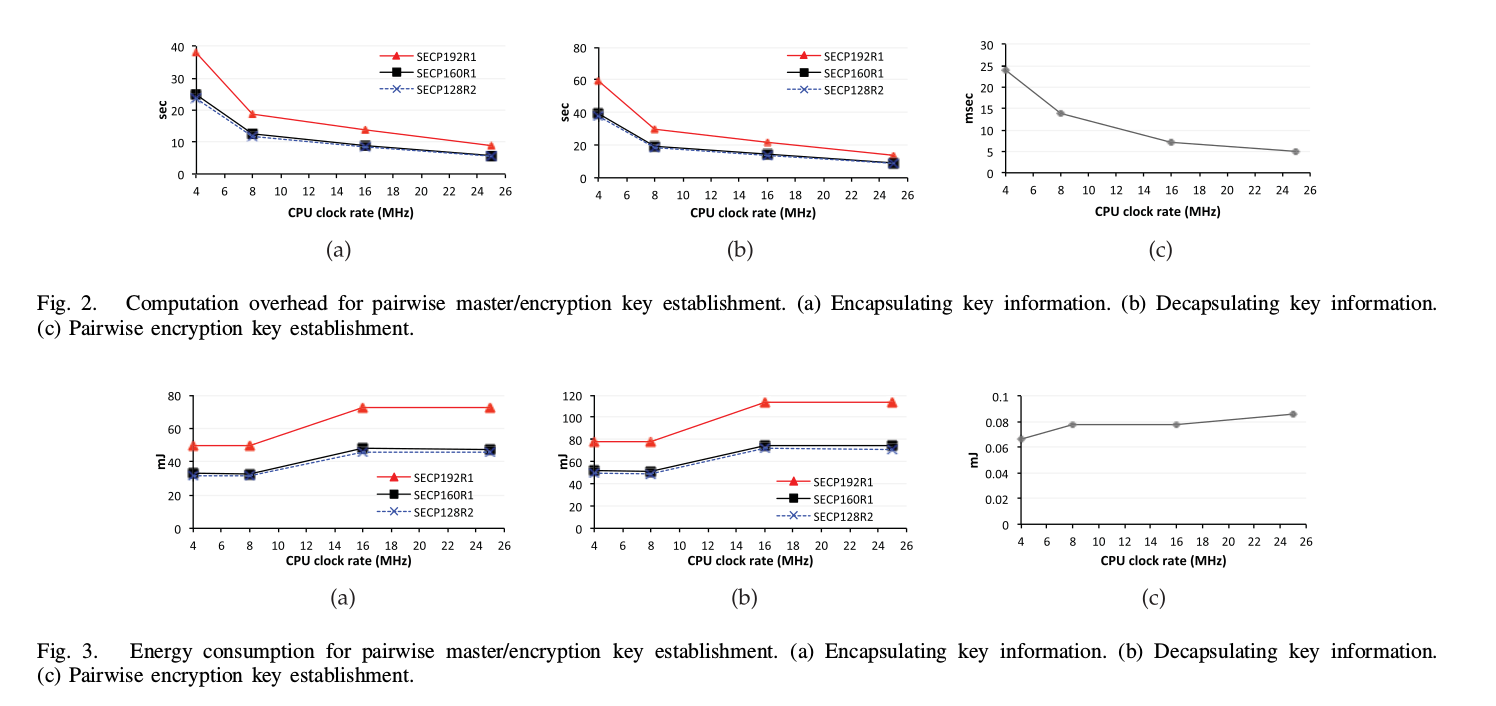
\includegraphics[width=1.0\textwidth,natwidth=1496,natheight=706]{./figures/figure-06.png}
  \end{center}
  \caption{Performance of ECC algorithm's \cite{seo;etal:2015}}
  \label{fig:label}
\end{figure}
The next figure shows the network power consumption for variable security configurations based on either a random walk or a Manhattan mobility model. The simulations are based on a 400 x 400 m grid, with 100 L-Sensors and 25 H-Sensors deployed. The configurable security settings are a) \emph{tbackoff} (how many seconds from a node leave until cluster heads update the cluster key, and b) \emph{thold} (how many seconds the pairwise key is kept in memory).\par
\begin{figure}[ht]
	\begin{center}
  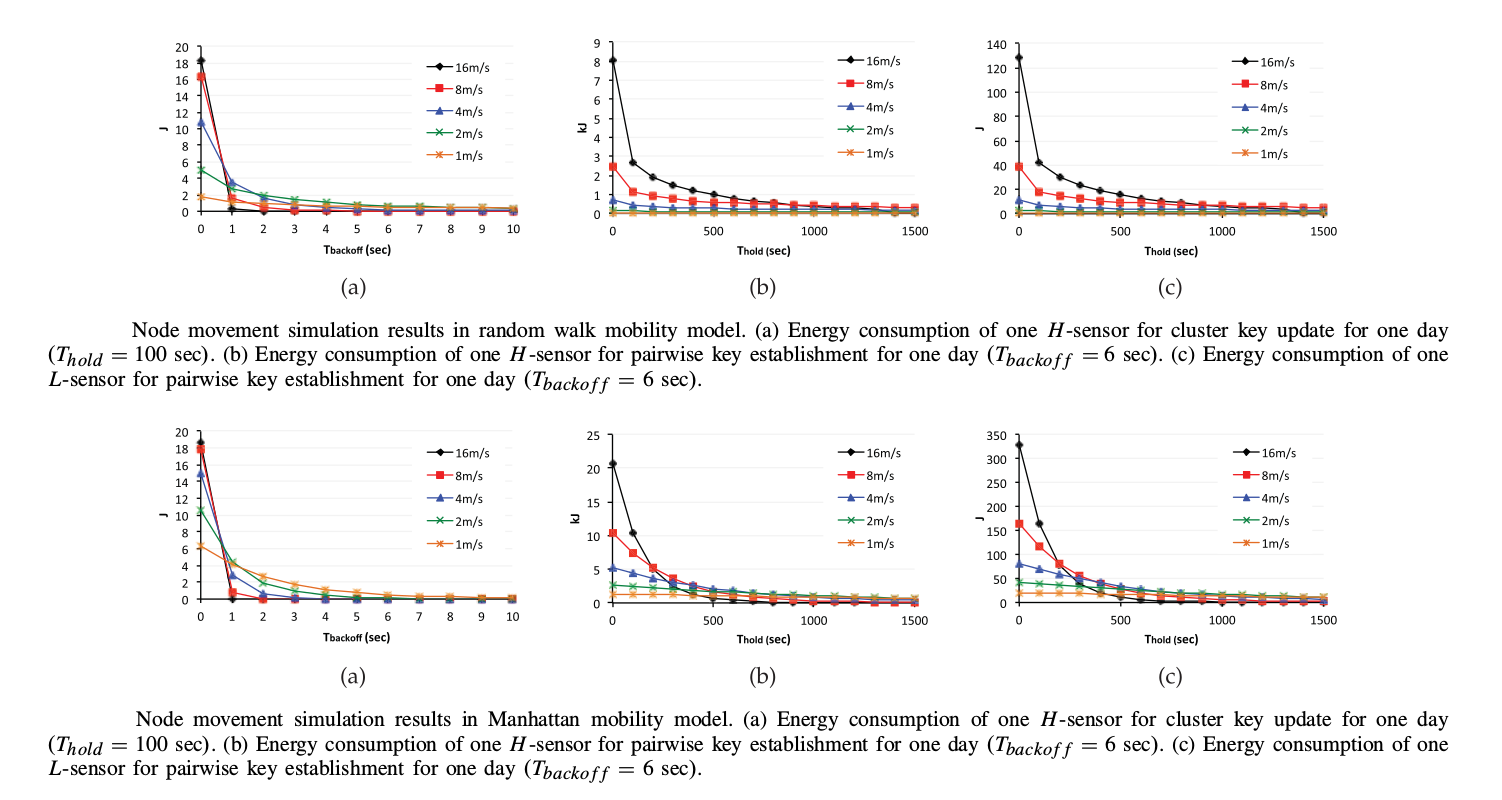
\includegraphics[width=1.0\textwidth,natwidth=1502,natheight=800]{./figures/figure-07.png}
  \end{center}
  \caption{Performance Impact of Security Configurations \cite{seo;etal:2015}}
  \label{fig:label}
\end{figure}
The larger tbackoff, the lower the security level is. Thus, there is a tradeoff between the security level and the energy consumption of the H -sensor. However, at high speeds (>16 m/s), tbackoff should be less than 1s in order to minimize the number of cluster key updates. At low speeds, 1, 2 or 3 seconds are a reasonable choice for the H -sensors \cite[ pp. 382]{seo;etal:2015}.\par 
The effect of thold increases as the node speed increases. As thold increases, the energy consumption decreases because in the event that the L-sensors return to the old clusters before the timers expire, no new pairwise master key establishment is necessary \cite[ pp. 382]{seo;etal:2015}.\par
Overall, this example scenario implementing a certificateless key management scheme for WSN's demonstrates how it is required to make tradeoffs between security and performance on a high level, whenever a WSN is built. The main question therefore always has to be, how sensitive the data aggregated and forwarded by the network is, and what protection efforts are necessary in order to protect that data.
\subsection{Trust-based Enforcement of Security Policies}
Our second solution aims to optimize resource consumption for security policies. The \emph{Trust Based Enforcement of Security Policies}, or TESP, is designed and presented by Robert Vigo, Alessandro Celestini, Francesco Tiezzi, Rocco de Nicola, Flemming Nielson, and Hanne Riis Nielson\cite{vigo;etal:2014}. This group aims to dynamically determine the perfect balance between resource consumption and security strength through a system of reputations. Put in their own words, they "propose a modelling language and a framework in which security checks can be relaxed or strengthened to save resources or increase protection, on the basis of trust relationships among communicating parties. Such relationships are automatically derived through a reputation system, hence adapt dynamically to the observed behavior of the parties and are not fixed a priority \cite{vigo;etal:2014}.\par
The authors define security polices as "fixed rules concerning actions that have to be executed whenever given conditions are met". The situations in which the security policies are utilized are often highly dynamic and decisions may depend on factors unknown during the design. This is the case when the adversaries are humans or when the system in question is highly limited in resources - for wireless latter networks, the latter is an inherent issue. The authors address the dynamic nature of threats in networks by allowing the probability of strengthening a policy to change as we gain information: "the probabilistic enforcement of security policies can account for relaxing or strengthening a security check, aiming at saving re- sources or increasing protection. In order to react to a dynamic environment, the probability to undertake, relax, or strengthen a given security measure cannot be fixed a priority... but depends on our knowledge of the past and on our expectations for the future" \cite{vigo;etal:2014}.\par
The system uses a probabilistic reputation systems, where trust is quantified in probabilistic terms. Communicating parties rate each other after every interaction and then use rates to calculate a reputation score, which is used to manage future interactions. The authors add that the main advantage of reputation systems is that "they permit computing the probability that a policy is enforced as the system evolves and according to its observed behaviour. This leads to the notion of trust-based enforcement of security policies. The trust we put on the involved parties at a given time can be used to determine the actual enforcement of security policies" \cite{vigo;etal:2014}.\par
With this system in place, policies can be relaxed to save resources: expensive checks can be skipped or relaxed with interacting with a party that has shown fair behavior in the past. On the contrary, we can strengthen a policy when interacting a party we don't trust, or we can limit exchange of critical information to highly-trusted parties. \par
The group's solution to the challenge of modelling such a system is TESP (Trust-based Enforcement of Security Policies), a "calculus inspired by [DTU Compute, Technical University of Denmark], that enriches the StoKlaim \cite{sen:2009} formalism with probabilistic aspects for security policies and with primitives for managing reputation scores. . . . The main technical challenge addressed in this work is the integration of all these elements (in particular, probabilistic aspects, security policies, and reputations) in a uniform framework. . . . TESP (Trust-based Enforcement of Security Policies) is a distributed process calculus which can be used to model security policies and their probabilistic enforcement, relying on a reputation system to infer probabilities. The calculus, displayed in Table 1, enriches (a subset of) StoKlaim with primitives for handling reputations and inherits the aspect-oriented mind-set of AspectKP for the design of security policies."\cite{vigo;etal:2014}.\par
\begin{figure}[ht]
	\begin{center}
  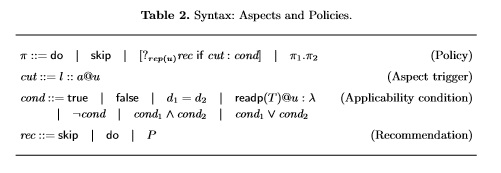
\includegraphics[width=1.0\textwidth,natwidth=501,natheight=173]{./figures/figure-03.jpg}
  \end{center}
  \caption{Syntax: Aspects and Policies \cite{vigo;etal:2014}}
  \label{fig:label}
\end{figure}
The base station is in charge of receiving readings and sending them to the central server. Once the signature check is successfully passed, the sensor reading is forwarded. As described by the authors, the process "consumes a check request, compares the signature with the source locality and sends a Boolean value representing the result of the comparison to the requester. In case the check fails, i.e., the message is corrupted, the base station discards it, otherwise it is forwarded to the server." The sensor receives a positive score if the check succeeds and a negative score if it fails. The reputation score is set to the number of positive interactions divided by the total number of interactions. This naturally raises the question - what is the score of each node in the beginning? To be safe, the score of all nodes is set to 0, where 0 is complete distrust and 1 is complete trust. \par
With a reputation system in place, the base station chooses for each new interaction whether no policy is enforced (action denied at source), one policy is enforced (action allowed at source and no policy at target), or two policies are enforced (both at source and target). This decision is made based upon the given threshold of interest. In the following table, we can see the probabilities of forwarding a corrupt message for different thresholds. As the authors point out, "we observe that the probability of satisfying the formula is strictly related to the sensor's behaviour and to the threshold value. In particular, it is not always true that the better the behaviour of the sensor, the lower the probability of forwarding corrupted messages, as one might expect. For th = 1\% the best result - that is, the lowest probability of sending more than 1\% corrupted messages - is achieved when the sensor's behaviour is the worst ($\theta$ = 0.2). This is due do to the fact that messages from trusted parties are seldom checked, yielding a higher number of forwarded messages". After simulating the process with SAM, two figures were ploted - the first with the ration between the number of unchecked and forwarded messages, and the second with the number of corrupted and forwarded messages.\par

\begin{figure}[ht]
	\begin{center}
  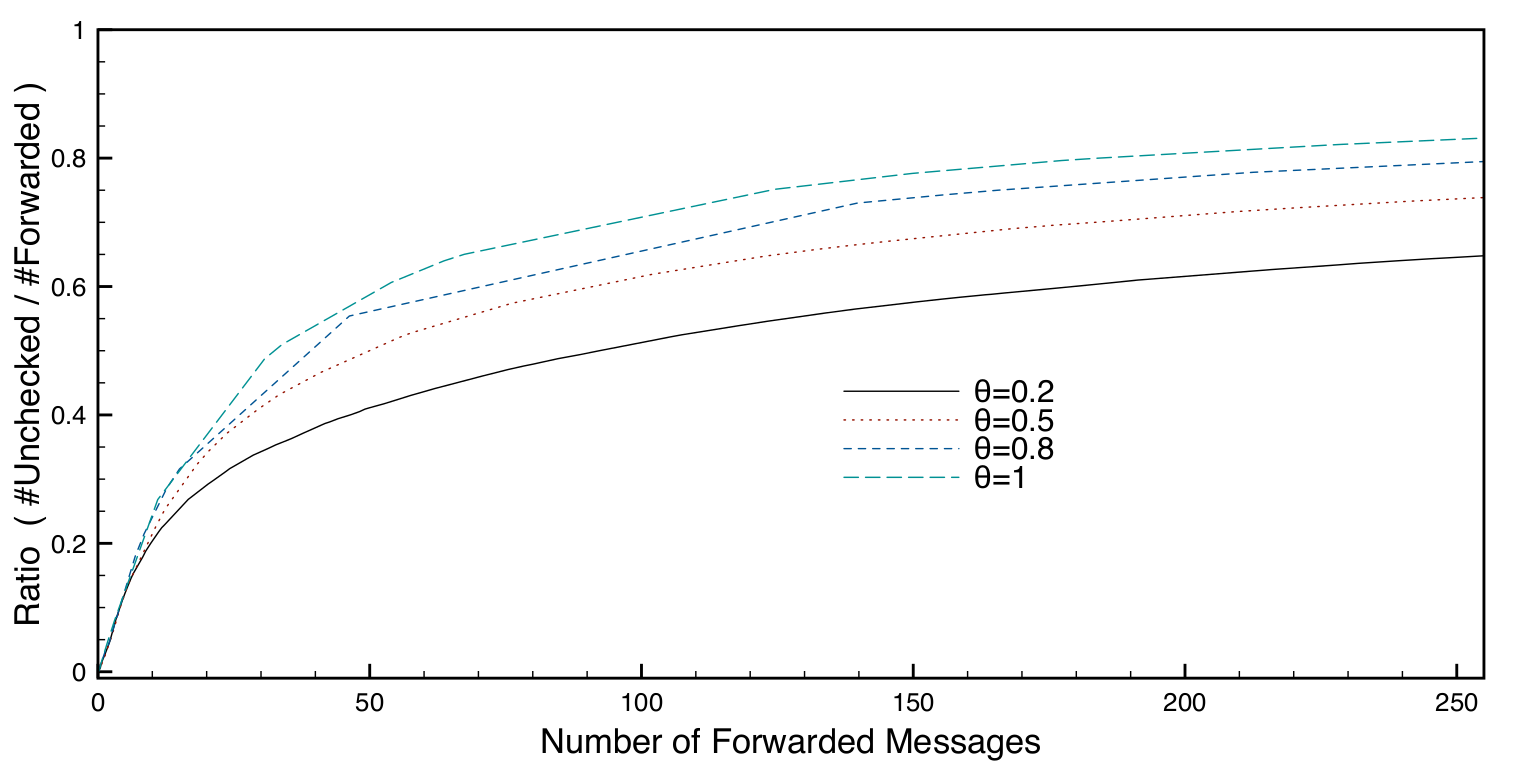
\includegraphics[width=0.8\textwidth,natwidth=631,natheight=345]{./figures/figure-04.png}
  \end{center}
  \caption{Ratio between unchecked and forwarded messages \cite{vigo;etal:2014}}
  \label{fig:label}
\end{figure}

As we expect in Figure 4, we see that the better the sensor behavior, the higher the ratio of unchecked messages, and thus the more resources saved. However, Fig. 5 seems not to confirm the results of the model checking analysis: the ratio of corrupted messages over the forwarded is lower for $\theta$ = 0.8 than for $\theta$ = 0.2. 

\begin{figure}[ht]
	\begin{center}
  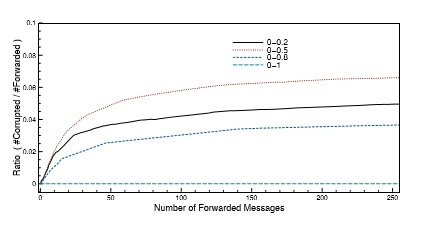
\includegraphics[width=0.8\textwidth,natwidth=429,natheight=239]{./figures/figure-05.jpg}
  \end{center}
  \caption{Ratio between corrupted and forwarded messages \cite{vigo;etal:2014}.}
  \label{fig:label}
\end{figure}
Nonetheless, as the authors state, we "observe that the simulation computes an average value, while the model checking algorithm estimates the probability of exceeding a threshold. Hence, we can conclude that on average the ratio between corrupted and forwarded messages is lower for $\theta$ = 0.8, but the probability that the number of corrupted messages exceeds a percentage of the forwarded messages is lower for $\theta$ = 0.2" \cite{vigo;etal:2014}. This is due to the decreasing number of checks that are performed for $\theta$ = 0.8, and to the fact that the model checking analysis has a temporal horizon: for a fixed time limit t, the total number of messages processed by the system is higher for $\theta$ = 0.8 than for $\theta$ = 0.2.\par
Through this reputation system, we dynamically adjust the probability that a security policy will be strengthened or weakened. In this way, we find an optimized balance between security strength and resource usage while adapting to the current environment and security needs of the WSNs. \par

\subsection{Dynamic Reconfiguration - Inter-trust \& Famiware}
This section introduces the third apprach for the Security policy re-configuration. Here we first discuss the Dynamic Software Product Lines in FamiWare. It is basically about dynamic software product lines and dynamic security frameworks. We focus on how these techniques are used in FamiWare and INTER-TRUST, respectively. In further part of the section we give the integration of Famiware and Inter-trust Framework and answer of "Why Inter-trust framework is nesserory to achive the Dynamic reconfiguration of Security policies". 
\subsubsection{Dynamic Software Product Lines in FamiWare}
The WSN sensor nodes have low level programming, limited capabilities and different protocols for routing. This means that the system needs some self-adaptation and self-protection mechanisms, which can be achieved by using the dynamic adaptation of the algorithms used for security. Dynamic software product lines (DSPLs) represent an emerging field that is producing software products capable of adapting to requirements that change at runtime. DSPLs allow managing the software adaptation so they can be the key technologies to consider for building self-protected WSN with Different approaches for each configuration challenge.\par
The Dynamic approach can be applied by using the DSPL approach (FamiWare Middleware) and the Inter-trust framework in the Security reconfiguration. This is to tackle the existing security issues, by making each node the decision maker for adapting the security policies according to the physical environment.\par
"Dynamic software product lines (DSPLs) represent an emerging field that is producing software products capable of adapting to requirements that change at runtime" \cite{Pinto;etal:2013}. A sensor node is a composition of features from asset of common and variable features, where the variable features may vary at runtime. Therefore, the products have the capacity to reconfigure themselves by binding variation points at runtime, several times, in accordance with the changes in the environment. "DSPLs uses variability model to specify the nodes that can be changed at runtime. In the solution, the use of non-standard languages or formalisms is avoided, and we use the Common Variability Language (CVL) proposed as the standard by the Object Management Group (OMG)" \cite{Pinto;etal:2013}. CVL is a domain-independent language for specifying and resolving variability. The CVL variability models allow modeling the variability separately from the base model, but both the variability and the base models are connected and can be managed using the same tool. The main characteristics of CVL are used to model the FamiWare variability model. The dynamic reconfiguration is defined as replacing one algorithm with other depending on the environment change. As the context changes the nodes are bound to change to get the perfect configuration. Therefore, using the CVL approach, we automatically generate both the initial configuration and also the successive adapted configurations. \par
"The inherent heterogeneity and the variability of WSNs are modeled in FamiWare using CVL variability models (i.e., the VSpec trees). FamiWare proposes the customization of the piece of software related to the middleware platform that is deployed in each device of the WSN according to: \par
\begin{enumerate}
	\item  the device features (device [1..*] feature in Figure 1 with a 1..* cardinality to represent the different devices in the system); 
	\item the application requirements (application feature); and 
	\item the global characteristics of the network used to connect the different devices (network feature)"\cite{Pinto;etal:2013}.
\end{enumerate}
Each device is having some other features, and can be represented by its types and the FamiWare services that need to be instantiated in that particular device according to the applications requirements. Regarding their types, devices can be of high capacity computers and other sensors. For FamiWare, the variability is decided for each device, so the FamiWare services instantiated in each device can be different. Among other services, FamiWare is composed of three optional services: monitoring, context awareness and reconfiguration. The FamiWare is checked on different types of characteristics such as memory consumption, battery level, and status of network connections.\par
\subsubsection{Dynamic Security Frameworks: INTER-TRUS}
\begin{figure}[ht]
	\begin{center}
  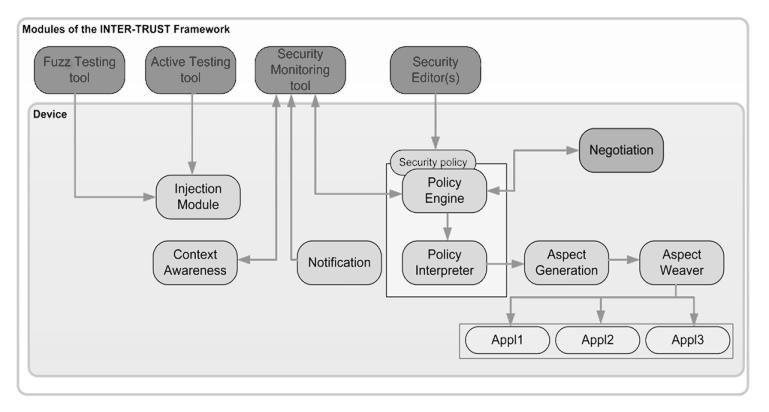
\includegraphics[width=1.0\textwidth,natwidth=769,natheight=412]{./figures/figure-02.png}
  \end{center}
  \caption{The INTER-TRUST framework \cite{ayed;etal:2013}.}
  \label{fig:label}
\end{figure}

The Security framework is a reusable set of modules that can be customized to develop trustworthy applications. The frame work describes the functionalities of each module that can be distinguished in a security framework. There are two different frameworks .\par

\begin{enumerate}
	\item  Framework that contains a set of modules which implements authorization, authentication, privacy and other such security concerns.
	\item Framework contains modules which deploys the security applications.
\end{enumerate}
Among these modules the framework can incorporate specific modules to adapt the security level of application at runtime. In this scenario we use Dynamic security framework.
The INTER-TRUST framework is a dynamic security framework \cite{ayed;etal:2013} to support trustworthy applications based on the enforcement and dynamic adaptation of security policies. In the INTER-TRUST framework, security policies are first specified using a security editor (e.g., MotOrBac, an Organization-Based Access Control policy editor) and then negotiated between the different parties in a communication using a negotiation module. When the security requirements change at runtime, the security policies are (re)negotiated. The negotiated security policy is then analyzed and interpreted by the policy engine and the policy interpreter modules. These modules are responsible for identifying changes in the security policy that require adapting the security concerns (e.g., authentication, encryption, etc.) deployed inside the application dynamically, at runtime.\par

\subsubsection{Integration of FamiWare and INTER-TRUST}
FamiWare is a family of middlewares specially designed and implemented for dealing with the heterogeneity of WSNs devices. It also provides a mechanism to be reconfigured at runtime when the context changes. However, it does not focus on providing security. Therefore, if we want to extend FamiWare with the benefits provided by the INTER-TRUST framework, the first thing to do is to integrate INTER-TRUST into the FamiWare family. There are two main steps for integration of the two application models, the first step is the integration of the INTER-TRUST modules and the INTER-TRUST security concerns into the FamiWare product line. This implies the extension of both the variability model and the base model of FamiWare. \par
\subsubsection{Dynamic Reconfiguration of Security in FamiWare}
FamiWare uses VSpec tree at runtime to handle the reconfiguration and the task to change the policies as the context changes. It uses models@run.time \cite{blair;bencomo:2009} approach to interpret the reconfiguration plans with the task to complete for switching from the middleware configuration to the new configuration of policy. These changes are performed taking care of the architectural design so, most of the time it fits the system restrictions. Other approaches for reconfiguration is working on code level, so the issue of hard-coding arise, so the competence between the new code and the models used for design is lost. This makes it difficult to claim that the reconfiguration applied at one node will work properly for whole network, when it is deployed at each node.\par

\section{Evaluation \& Discussion}
This Section talks mainly about the Challenges and Approaches for Inter-trust \& FamiWare. Here we present the different cases and the problem areas with respect to the existing senarios with the Wireless Sensor Networks, and how the given appraoch gives the solution for it.
\subsection{Challenges and Approaches for Inter-trust \& FamiWare}
The main challenges that need to be taken into account in order to add security to WSNs and to dynamically (re)configure the security level at runtime, can be described as follows:
\begin{enumerate}
	\item  "Build secure applications that run on heterogeneous nodes with limited capabilities" \cite{Pinto;etal:2013}.\par
As we have seen in WSNs each node is different and provides different services. At each node there are different devices and applications installed that makes the node heavier and unable to adapt the different algorithms. Here we are giving the solution to this by integrating the INTER-TRUST framework and FamiWare security product lines. The nodes should not carry other things than the algorithms to switch as the context changes.
	\item  "Dynamic negotiation of security policies for WSNs.\par
	The conditions of the running environment of the WSNs applications could change. Then, the security policies may need to be adapted to the new conditions. This adaptation requires a previous negotiation between the different parts of the application" \cite{Pinto;etal:2013}. The solution we are presenting using the same integration of approaches. By this integration FamiWare middle ware gives the platform for dynamic negotiation for security policies for the sensor nodes that are already included into the FamiWare.
	\item  "Monitor the changes in the context.\par
	These changes can be general (e.g., changes in the amount of memory or the battery level available) or can be specific to security. In order to react to these changes, the environment needs to be monitored" \cite{Pinto;etal:2013}. The solution can be again obtained from choosing the different essential monitoring features available in both the applications as Inter-trust and FamiWare. Here we will only choose those monitoring modules which are essential for particular node, by choosing only those important components from Inter-Trust which is not present in FamiWare.  
	\item "Define a dynamic reconfiguration service to endow applications with self-protection.
When the environment or the security requirements change at runtime, the system must be self-protected to maintain a proper and secure functioning" \cite{Pinto;etal:2013}. \par
As WSNs are composed of a large number of tiny devices, the self-protection mechanism should consume the least number of resources as possible" \cite{Pinto;etal:2013}. Our approach says, it is proven that the FamiWare pays special attention to the efficiency of the nodes. The resource consumption of Famiware is optimal for certain typical type of sensors, and it is also scalable to a number of nodes.
\end{enumerate}
\subsection{Conclusion}
In this paper we have discussed the increasing usages of WNS and we discussed an example of ITS for explaining the current situation of WSN. The paper has presented three diffrent solutions in further sections for the Dynamic re-configuation of security policies.\par
In the first section, the major attack venues and defense mechanisms appropriate in WSNs were introduced, along with an outline as to why it is crucial to have these security mechanisms in place. \par
In the next section, we provided practical examples of complete implementations for providing end-to-end security in dynamic wireless sensor networks.\par
In conclusion, our hope is that the reader of this text has received a general overview of the security mechanisms that can be deployed in a WSN, and is capable of choosing the appropriate protections for his or her use case. With that, we would like to close with the following quote, which already hints at a future where WSN's are distributed all over the world: \par
"Sensor networks are set to become a truly pervasive technology that will affect our daily lives in important ways. We cannot deploy such a critical technology, however, without first addressing the security and privacy research challenges to ensure that it does not turn against those whom it is meant to benefit" \cite[ pp. 101]{chan;perrig:2003}.\par


%%%%%%%%%%%%%%%%%%%%%%%%%%%%%%%%%%%%% commented start
\iffalse

\section{Acronyms \& Terminology}
\FloatBarrier
\begin{table}[H]
    \caption{Acronyms}
  	\begin{center}
    \begin{tabular}{|c|c|} \hline
	        Acronym & Definition \\ \hline\hline
	        \si{\micro}TESLA & micro version of timed efficient streaming loss-tolerant authentication protocol\\ \hline
	        AES & Advanced Encryption Standard \\ \hline
	        BS & base station \\ \hline
	        CDA & concealed data aggregation  \\ \hline
	        CL-EKM & certificateless effective key management \\ \hline
	        CL-HSC & pairing-free certificateless hybrid signcryption scheme \\ \hline
	        CSA & context speed advisory \\ \hline
	        CVL & Common Variability Language \\ \hline
	        D-H & Diffie Hellman key agreement protocol \\ \hline
	        DoS & Denial of Service \\ \hline
	        DSPLs & Dynamic software product lines \\ \hline
	        ECC & Elliptic Curve Cryptography  \\ \hline
	        ESPDA & energy-efficient secure pattern-based data aggregation \\ \hline
	        GROW & Greedy random walk protocol. \\ \hline
	        HSC & homomorphic stream cipher\\ \hline
	        IDS & Intrusion Detection System \\ \hline
	        ID-PKC & identity-based public key cryptography  \\ \hline
	        IHOP & interleaved hop-by-hop authentication \\ \hline
	        INENS & intrusion tolerant routing protocol in wireless sensor networks \\ \hline
	        KDC & key distribution center \\ \hline
	        LIDS & local intrusion detection system \\ \hline
	        OBU & on-board unit \\ \hline
	        OMG & Object Management Group \\ \hline
	        PET & personalized trust model called\\ \hline
	        PH & privacy homomorphism \\ \hline
	        PKC & public key cryptography \\ \hline
	        RSA & Ron Rivest, Adi Shamir, and Leonard Adleman (Algorithm) \\ \hline
	        SDDA & secure differential data aggregation \\ \hline
	        SIA & secure information aggregation \\ \hline
	        SINP & securing in-network processing \\ \hline
	        SPINS & security protocols for sensor networks \\ \hline
	        SNEP & secure network encryption protocol \\ \hline
	        TESP & Trust Based Enforcement of Security Policies \\ \hline
	        TRANS & trust routing for location aware sensor networks \\ \hline
	        WDA & witness-based data aggregation \\ \hline
	        WSN & wireless sensor network \\ \hline
	  \end{tabular}
	  \end{center}
  \end{table}
\FloatBarrier

%%%%%%%%%%%%%%%%%%%%%%%%%%%%%%%%%%%%% commented end
\fi


\begin{thebibliography}{99}
\bibitem {leitfaden} Martin Waldburger, Patrick Poullie, Burkhard Stiller: \emph{Guideline for Seminar Reports}, Communication Systems Group, Department of Infromatics, University of Zurich, January 2013. \url{http://www.csg.uzh.ch/teaching/guideline-seminar-report-v05.pdf}.
\bibitem {chan;perrig:2003} Chan, Haowen, and Adrian Perrig: \emph{Security and privacy in sensor networks}, Computer 36.10 (2003): 103-105. \url{http://www.netsec.ethz.ch/publications/papers/ieee-secure-sensor-nets.pdf}.
\bibitem {wang;attebury;ramamurthy:2006} Y. Wang, G. Attebury, and B. Ramamurthy: \emph{A survey of security issues in Wireless Sensor Networks}, IEEE Communications Surveys and Tutorials, Vol. 8, No. 2, pp. 2-23, 2006.
\bibitem {sen:2009} J. Sen: \emph{A Survey on Wireless Sensor Network Security}, International Journal of Communication Networks and Information Security (IJCNIS), vol.1, no.1, pp. 55-78, August 2009.
\bibitem {itu-t:2012} ITU-T: \emph{Y2060 - Overview of the Internet of things}, 2012. \url{https://www.itu.int/rec/T-REC-Y.2060-201206-I}.
\bibitem {pinto;etal:2015} M. Pinto, N. Gamez, L. Fuentes, M. Amor, J.M. Horcas, I. Ayala: \emph{Dynamic Reconfiguration of Security Policies in Wireless Sensor Networks}, Sensors, vol. 15, 2015, pp. 5251-5280. DOI: 10.3390/s150305251. \url{http://www.mdpi.com/1424-8220/15/3/5251/htm}.
\bibitem {seo;etal:2015} Seo, Seung-Hyun, Jongho Won, Shabana Sultana, and Elisa Bertino. \emph{Effective key management in dynamic wireless sensor networks}, Information Forensics and Security, IEEE Transactions on 10, no. 2 (2015): 371-383. \url{http://docs.lib.purdue.edu/cgi/viewcontent.cgi?article=1640&context=ccpubs}.
\bibitem {vigo;etal:2014} Vigo, Roberto, Alessandro Celestini, Francesco Tiezzi, Rocco De Nicola, Flemming Nielson, and Hanne Riis Nielson. \emph{Trust-based Enforcement of Security Policies}, In Trustworthy Global Computing, pp. 176-191. Springer Berlin Heidelberg, 2014. \url{http://citeseerx.ist.psu.edu/viewdoc/download?doi=10.1.1.431.4963&rep=rep1&type=pdf}.
\bibitem {erfani;etal:2015} Erfani, Seyed Hossein, Hamid HS Javadi, and Amir Masoud Rahmani. \emph{A dynamic key management scheme for dynamic wireless sensor networks}, Security and Communication Networks 8, no. 6 (2015): 1040-1049.
\bibitem {Pinto;etal:2013} 1) M\'{o}nica Pinto *, Nadia G\'{a}mez , Lidia Fuentes , Mercedes Amor , Jos\'{e} Miguel Horcas and Inmaculada Ayala. \emph{Dynamic Reconfiguration of Security Policies in Wireless Sensor Networks}. Sensors 2013, 15(3), 5251-5280. [Google Scholar]
\bibitem {blair;bencomo:2009} Gordon Blair and Nelly Bencomo, Lancaster University Robert B. France, Colorado State University. \emph{models@run.time}. 2009 IEEE, IEEE Computer Society. [IEEE xplore]
\bibitem {ayed;etal:2013} 3) Ayed, S. Telecom Bretagne, Rennes, France Idrees, M.S. ; Cuppens-Boulahia, N. ; Cuppens, F. ; Pinto, M. ; Fuentes, L.\emph{Security Aspects: A Framework for enforcement of security policies using AOP}.Signal-Image Technology \& Internet-Based Systems (SITIS), 2013 International Conference on. [IEEE xplore]
\bibitem {rabin:1979} M.O. Rabin, \emph{Digitalized Signatures and Public-Key Functions as Intractable as Factorization}, Cambridge, MA, Technical Report, 1979.
\bibitem {hoffstein;etal:1998} J. Hoffstein, J. Pipher, and J.H. Silverman, \emph{Ntru: A ring-basedpublic key cryptosystem}, In Proceedings of the 3 rd International Symposium on Algorithmic Number Theory, London, Springer-Verlag, 1998, pp. 267-288.
\bibitem {RSA:1983} R.L. Rivest, A. Shamir, and L. Adleman, \emph{A method for obtaining digital signatures and public-key cryptosystems}, Communications of the ACM, Vol. 26, No. 1, pp. 96-99, 1983.
\bibitem {miller:1986} V.S. Miller, \emph{Use of elliptic curves in cryptography}, In Lecture Notes in Computer Sciences: 218 on Advances in Cryptology-CRYPTO 85, New York, Springer-Verlag, 1986, pp. 417-426.
\bibitem {kobiltz:1987} N. Kobiltz, \emph{Elliptic curve cryptosystems}, Mathematics of Computation, Vol. 48, pp. 203-209, 1987.
\bibitem {deng;etal:2003} J. Deng, R. Han, and S. Mishra, \emph{Security support for in-network processing in wireless sensor networks}, In Proceedings of the 1st ACM Workshop on Security of Ad hoc and Sensor Networks, New York, ACM Press, 2003, pp. 83-93.
\bibitem {cam;etal:2003} H. Cam, D. Muthuavinashiappan, and P. Nair, \emph{ESPDA: Energy-efficient and secure pattern-based data aggregation for wireless sensor networks}, In Proceedings of IEEE Sensors, Toronto, Canada, October 2003, pp. 732-736.
\bibitem {cam;etal:2004} H. Cam, S. Ozdemir, H.O. Sanli, and P. Nair, \emph{Sensor Network Operations}, Wiley, 2004, Chapter: Secure Differential Data Aggregation for Wireless Sensor Networks.
\bibitem {cam;etal:2005} H. Cam, D. Muthuavinashiappan, and P. Nair, \emph{Energy-efficient security protocol for wireless sensor networks}, In Proceedings of IEEE VTC Conference, Orlando, Florida, October 2005, pp. 2981- 2984.
\bibitem {du;etal:2003} W. Du, J. Deng, Y.S. Han, and P.K. Varshney, \emph{A witness-based approach for data fusion assurance in wireless sensor networks}, In Proceedings of IEEE Global Telecommunications Conference, San Francisco, December 2003, pp. 1435-1439
\bibitem {girao;etal:2005} J. Girao, D. Westhoff, and M. Schneider, \emph{CDA: Concealed data aggregation for reverse multicast traffic in wireless sensor networks}, In Proceedings of IEEE International Conference on  Communications, Seoul, Korea, May 2005.
\bibitem {castelluccia;etal:2005} C. Castelluccia, E. Mykletun, and G. Tsudik, \emph{Efficient aggregation of encrypted data in wireless sensor network}, In Proceedings of ACM/IEEE Mobiquitous, San Diego, July 2005.
\bibitem {seshadri;etal:2004} A. Seshadri, A. Perrig, L. Van Doorn, and P. Khosla,\emph{SWATT: Software-based attestation for embedded devices}, In Proceedings of the IEEE Symposium on Security and Privacy, May 2004.
\bibitem {liang;shi:2005} Z. Liang and W. Shi, \emph{PET: A Personalized Trust model with reputation and risk evaluation for P2P resource sharing}, In Proceedings of the HICSS-38, Hilton Waikoloa Village Big Island, Hawaii, January 2005.
\end{thebibliography}

\end{document}
